%%%%%%%%%%%%%%%%%%%%%%%%%%%%%%%%%%%%%%%%%
% Beamer Presentation
% LaTeX Template
% Version 1.0 (10/11/12)
%
% This template has been downloaded from:
% http://www.LaTeXTemplates.com
%
% License:
% CC BY-NC-SA 3.0 (http://creativecommons.org/licenses/by-nc-sa/3.0/)
%
%%%%%%%%%%%%%%%%%%%%%%%%%%%%%%%%%%%%%%%%%

%----------------------------------------------------------------------------------------
%	PACKAGES AND THEMES
%----------------------------------------------------------------------------------------

\documentclass{beamer}

\mode<presentation> {

% The Beamer class comes with a number of default slide themes
% which change the colors and layouts of slides. Below this is a list
% of all the themes, uncomment each in turn to see what they look like.

%\usetheme{default}
%\usetheme{AnnArbor}
%\usetheme{Antibes}
%\usetheme{Bergen}
\usetheme{Berkeley}
%\usetheme{Berlin}
%\usetheme{Boadilla}
%\usetheme{CambridgeUS}
%\usetheme{Copenhagen}
%\usetheme{Darmstadt}
%\usetheme{Dresden}
%\usetheme{Frankfurt}
%\usetheme{Goettingen}
%\usetheme{Hannover}
%\usetheme{Ilmenau}
%\usetheme{JuanLesPins}
%\usetheme{Luebeck}
%\usetheme{Madrid}
%\usetheme{Malmoe}
%\usetheme{Marburg}
%\usetheme{Montpellier}
%\usetheme{PaloAlto}
%\usetheme{Pittsburgh}
%\usetheme{Rochester}
%\usetheme{Singapore}
%\usetheme{Szeged}
%\usetheme{Warsaw}

% As well as themes, the Beamer class has a number of color themes
% for any slide theme. Uncomment each of these in turn to see how it
% changes the colors of your current slide theme.

%\usecolortheme{albatross}
%\usecolortheme{beaver}
%\usecolortheme{beetle}
%\usecolortheme{crane}
\usecolortheme{dolphin}
%\usecolortheme{dove}
%\usecolortheme{fly}
%\usecolortheme{lily}
%\usecolortheme{orchid}
%\usecolortheme{rose}
%\usecolortheme{seagull}
%\usecolortheme{seahorse}
%\usecolortheme{whale}
%\usecolortheme{wolverine}

%\setbeamertemplate{footline} % To remove the footer line in all slides uncomment this line
%\setbeamertemplate{footline}[page number] % To replace the footer line in all slides with a simple slide count uncomment this line

%\setbeamertemplate{navigation symbols}{} % To remove the navigation symbols from the bottom of all slides uncomment this line
}

\usepackage{graphicx} % Allows including images
\usepackage{booktabs} % Allows the use of \toprule, \midrule and \bottomrule in tables
\usepackage[utf8]{inputenc}
\usepackage{multirow}

%----------------------------------------------------------------------------------------
%	TITLE PAGE
%----------------------------------------------------------------------------------------

\title[EP3]{EP3 - MAC0422} % The short title appears at the bottom of every slide, the full title is only on the title page

\author{João Gabriel e Juliano Garcia} % Your name
\institute[IME- USP] % Your institution as it will appear on the bottom of every slide, may be shorthand to save space
{
Instituto de Matemática e Estatística - USP \\ % Your institution for the title page
}
\date{} % Date, can be changed to a custom date

\begin{document}

\begin{frame}
\titlepage % Print the title page as the first slide
\end{frame}

\begin{frame}
\frametitle{Overview} % Table of contents slide, comment this block out to remove it
\tableofcontents % Throughout your presentation, if you choose to use \section{} and \subsection{} commands, these will automatically be printed on this slide as an overview of your presentation
\end{frame}

%----------------------------------------------------------------------------------------
%	PRESENTATION SLIDES
%----------------------------------------------------------------------------------------

%------------------------------------------------
\section{Estruturas}
%------------------------------------------------

\begin{frame}
\begin{center}
\huge Estruturas
\end{center}
\end{frame}

\begin{frame}
\frametitle{Estruturas de dados utilizadas}
\begin{itemize}
\item Linguagem: Python 3.6
\item Listas (built-in do python)
\item Lista Ligada (representação da memória)
\item Arquivos
\item Classes no geral (OOP)
\end{itemize}
\end{frame}

\begin{frame}
\frametitle{Decisões de implementação}
\begin{figure}
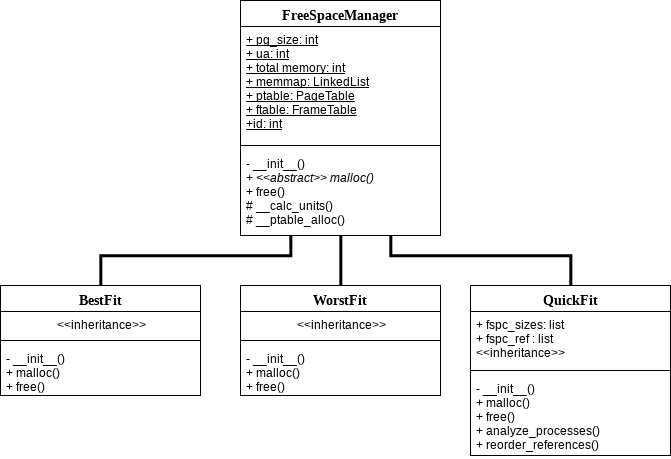
\includegraphics[scale=0.4]{class_fspc.png}
\end{figure}
\end{frame}

\begin{frame}
\frametitle{Decisões de implementação}
\begin{figure}
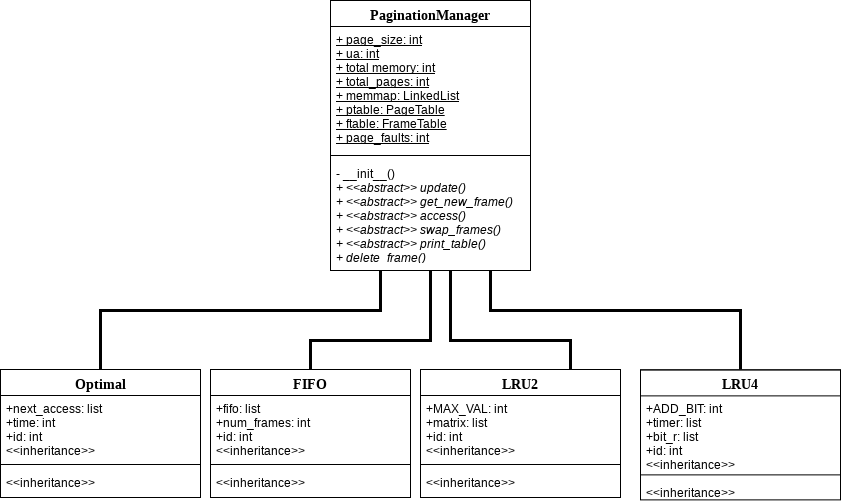
\includegraphics[scale=0.35]{class_paginators.png}
\end{figure}
\end{frame}

%-------------------------------------------------
\section{Gerenciamento de memória}
%-------------------------------------------------

\begin{frame}
\begin{center}
\huge Gerenciamento de memória
\end{center}
\end{frame}

\begin{frame}
\frametitle{Best Fit e Worst Fit}
\begin{itemize}
\item Best Fit: Percorre a lista ligada e encontra o nó cujo tamanho seja o menor possível e maior ou igual ao processo a ser alocado;
\item Worst Fit: Percorre a lista ligada e encontra o nó cujo tamanho seja o maior possível e maior ou igual ao processo a ser alocado;
\item A implementação de ambos é bastante similar e apenas o método de alocação diferente, ambos delegam a maioria das operações para a classe FreeSpaceManager.
\end{itemize}
\end{frame}

\begin{frame}
\frametitle{Quick Fit}
\begin{itemize}
\item Antes de começar a simulação, o Quick Fit analisa a lista de processos e cria uma lista com os 5 tamanhos mais requisitados (variável);
\item Cada tamanho tem uma lista com as referências dos nós daquele tamanho;
\item Se um tamanho é um dos mais requisitados, procura uma referência na lista específica daquele tamanho;
\item Senão, executa um First Fit, e atualiza a lista de listas tirando as referências que foram utilizadas;
\item Quando há compactação de memória, a lista de listas é zerada, e as novas referências são recalculadas e adicionadas novamente na lista.
\end{itemize}
\end{frame}

%-------------------------------------------------
\section{Paginação}
%-------------------------------------------------

\begin{frame}
\begin{center}
\huge Paginação
\end{center}
\end{frame}

\begin{frame}
\frametitle{Algoritmos de paginação}
\textbf{Optimal}:
\begin{itemize}
\item Implementa um contador regressivo para cada página, que é iniciado com o tempo restante para o próximo acesso do processo associado àquele quadro;
\item Se o processo não irá acessar mais a memória, o temporizador recebe infinito;
\item O quadro a ser retirado será o que tiver mais tempo restante no contador
\end{itemize}
\textbf{FIFO}
\begin{itemize}
\item Utiliza uma fila para gerenciar os quadros de página;
\item Quando uma página é colocada na memória física, ela é enfileirada;
\item Quando um page fault ocorre, a primeira página da fila é removida da memória física
\end{itemize}
\end{frame}

\begin{frame}
\frametitle{Algoritmos de paginação}
\textbf{LRU v2}
\begin{itemize}
\item Utiliza uma matriz de bits para gerenciar os quadros de página;
\item Cada linha da matriz é implementada como se fosse um número inteiro, e toda operação com as linhas é feita utilizando operadores bitwise
\end{itemize}
\textbf{LRU v4}
\begin{itemize}
\item Também implementa um contador para cada quadro, representado por um número inteiro;
\item O contador é envelhecido deslocando seus bits para a direita adicionando o bit R do quadro em seu bit mais significativo
\end{itemize}
\end{frame}

%------------------------------------------------
\section{Gráficos}
%------------------------------------------------

\begin{frame}
\begin{center}
\huge Gráficos
\end{center}
\end{frame}

\begin{frame}
\frametitle{Gráficos}
\begin{table}
\begin{tabular}{l l l l}
\toprule
\textbf{Algoritmo} & \textbf{Média} & \textbf{Variância} & \textbf{IC}\\
\midrule
Best fit   & 0.379 $\mu s$ & 0.0016 & [0.365, 0.394] \\
Worst fit  & 0.472 $\mu s$ & 0.0011 & [0.460, 0.485] \\
Quick fit  & 0.322 $\mu s$ & 0.0008 & [0.312, 0.333] \\
\bottomrule
\end{tabular}
\end{table}

\begin{table}
\begin{tabular}{l l l l}
\toprule
\textbf{Algoritmo} & \textbf{Média} & \textbf{Variância} & \textbf{IC}\\
\midrule
Optimal & 427 pfs & 0 & [427, 427] \\
FIFO    & 488 pfs & 0 & [488, 488] \\
LRU v2  & 474 pfs & 0 & [474, 474] \\
LRU v4  & 456 pfs & 0 & [456, 456] \\
\bottomrule
\end{tabular}
\end{table}
\end{frame}


\begin{frame}
\frametitle{Tempo para encontrar espaço livre}
\begin{figure}
% Mudar o gráfico
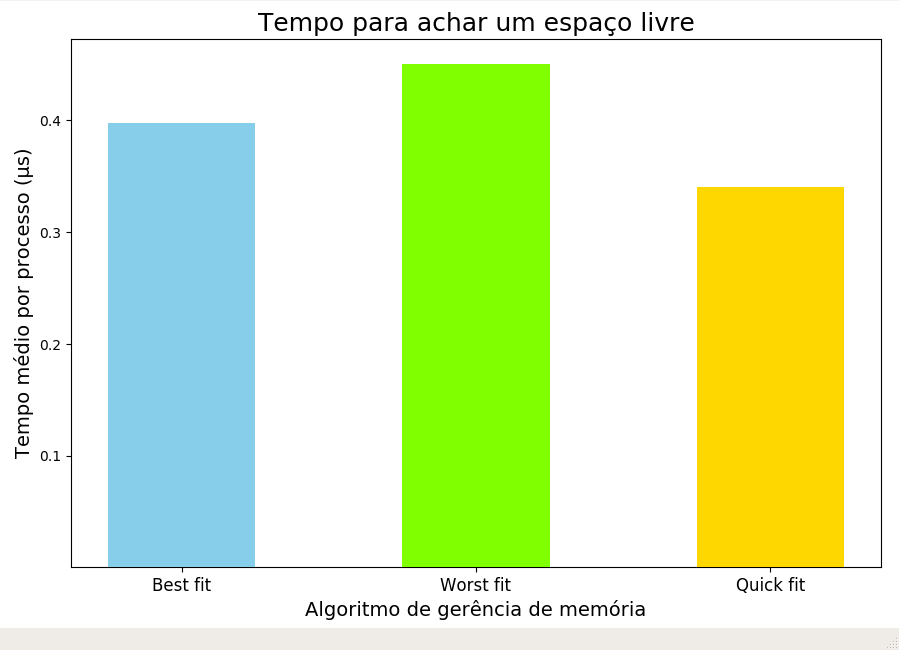
\includegraphics[scale=0.3]{alloc_time.png}
\end{figure}
\end{frame}

\begin{frame}
\frametitle{Page faults}
\begin{figure}
% Mudar o gráfico
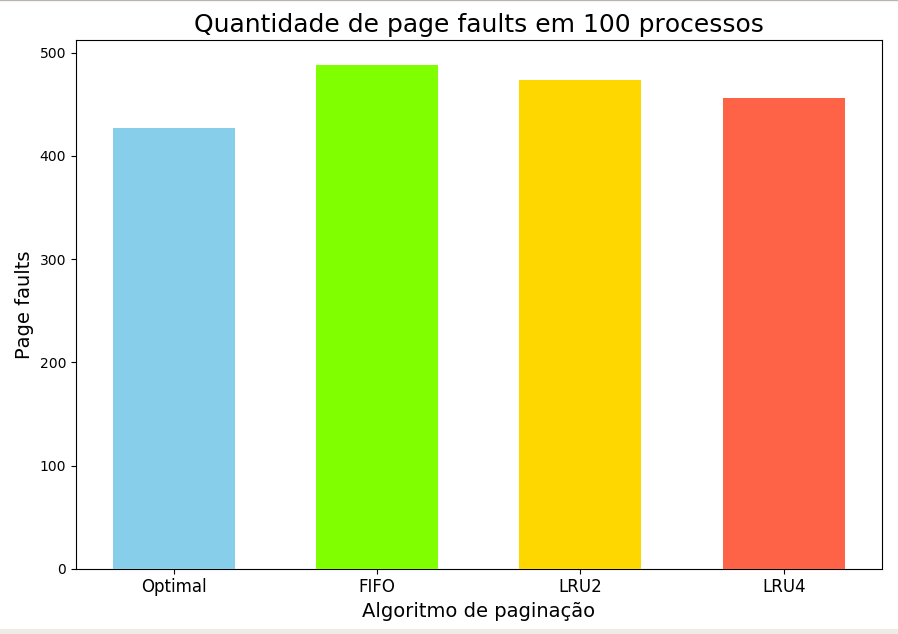
\includegraphics[scale=0.3]{page_faults.png}
\end{figure}
\end{frame}

\begin{frame}
\frametitle{Conclusões}
\begin{itemize}
\item Dentre os algoritmos de alocação, o mais rápido foi o quick fit, como esperado, seguido do best fit e por último o worst fit
\item O algoritmo de paginação com menos page faults foi o optimal, como esperado, seguido pelo LRU versão 4, que teve uma performance boa, e o LRU versão 2 e o FIFO levaram mais page faults
\item Com os resultados dos algoritmos de paginação, podemos perceber que não podemos evitar boa parte dos page faults, já que a diferença entre o melhor algoritmo (optimal) e o pior (FIFO) representa só 12\% dos page faults
\end{itemize}

\end{frame}

\begin{frame}
\frametitle{Bibliografia}
\footnotesize {
\begin{thebibliography}{99} % Beamer does not support BibTeX so references must be inserted manually as below
\bibitem[Sedgewick, Robert and Wayne, Kevin]{p1} Sedgewick, Robert and Wayne, Kevin
\newblock Algorithms, 4th Edition.
\bibitem[Tanenbaum, Andrew S.]{p1} Tanenbaum, Andrew S.
\newblock Modern Operating Systems, 4th Edition.
\end{thebibliography}
}
\end{frame}

% Blocks:
%\begin{block}{Block 1}
%Lorem ipsum dolor sit amet, consectetur adipiscing elit. Integer lectus nisl, ultricies in feugiat rutrum, porttitor sit amet augue. Aliquam ut tortor mauris. Sed volutpat ante purus, quis accumsan dolor.
%\end{block}

% Paragraph division: \\~\\

% Columns
%\begin{columns}[c] % The "c" option specifies centered vertical alignment while the "t" option is used for top vertical alignment

%\column{.45\textwidth} % Left column and width
%\textbf{Heading}
%\begin{enumerate}
%\item Statement
%\item Explanation
%\item Example
%\end{enumerate}

%\column{.5\textwidth} % Right column and width
%Lorem ipsum dolor sit amet, consectetur adipiscing elit. Integer lectus nisl, ultricies in feugiat rutrum, porttitor sit amet augue. Aliquam ut tortor mauris. Sed volutpat ante purus, quis accumsan dolor.

%\end{columns}

\end{document}